\section{Appendix}\label{appendix}

%%%%%%%%%%%%depends



\begin{figure}
\centering
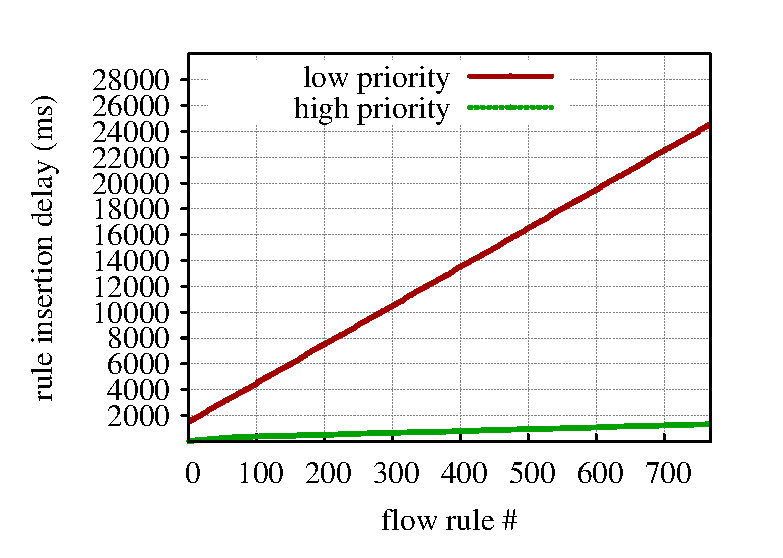
\epsfig{file=./figs/bcm_two_pri_outbound_burst.eps,width=0.5\textwidth}
\caption{Openflow rule priority's effects on proactive insertion delay. Measured on Broadcom switch. odd: 1, even: 2. Busrt mode (similar observations using controlled flow rates: 1/s, 10/s, 50/s, 100/s, and 200/s). High priority rules are inserted before the low priority rules}\label{bcm_compare_priority_simple1}
\end{figure}

\begin{figure}
\centering
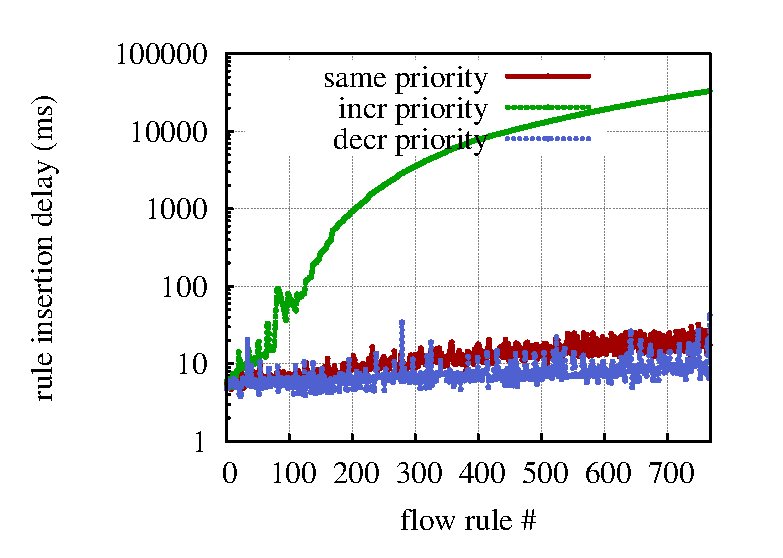
\epsfig{file=./figs/bcm_comp_pri_outbound_rate50.eps,width=0.5\textwidth}
\caption{Openflow rule priority's effects on proactive insertion delay. Measured on Broadcom switch. Averaged on 5 rounds. Insertion rate is 50 per sec.}\label{bcm_compare_priority_simple2}
\end{figure}


\begin{figure}
\centering
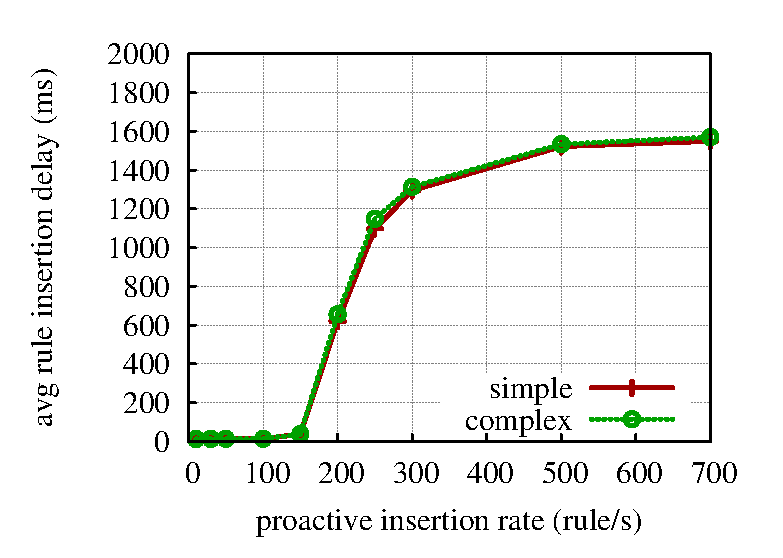
\epsfig{file=./figs/compare_complexity_bcm.eps,width=0.5\textwidth}
\caption{Openflow rule complexity's effects on proactive insertion delay. Measured on Broadcom switch.}\label{bcm_compare_complexity}
\end{figure}


\begin{figure*}
\subfloat[default table occupancy 100, insert another 50 rules\label{fig:bcm_outbound_rate_effect_1}]
  {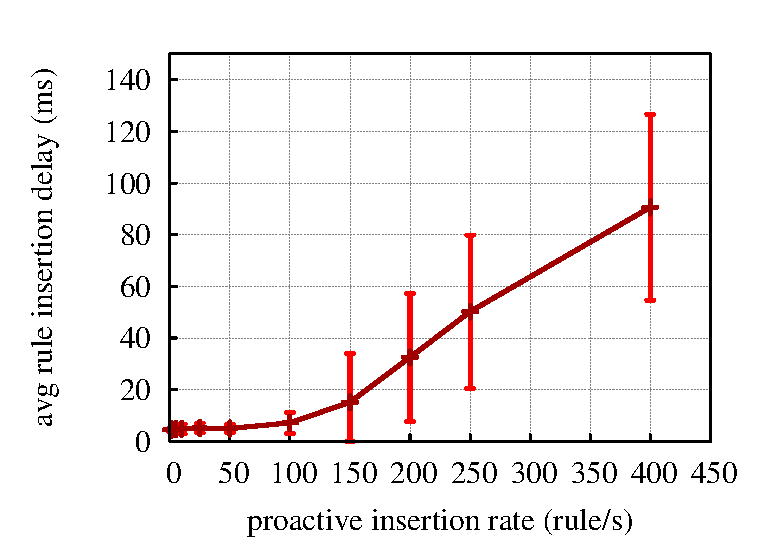
\includegraphics[width=.3\linewidth]{./figs/bcm_insertion_rate_effects_table100_rule50.eps}}\hfill
\subfloat[default table occupancy 100, insert another 300 rules\label{fig:bcm_outbound_rate_effect_2}]
  {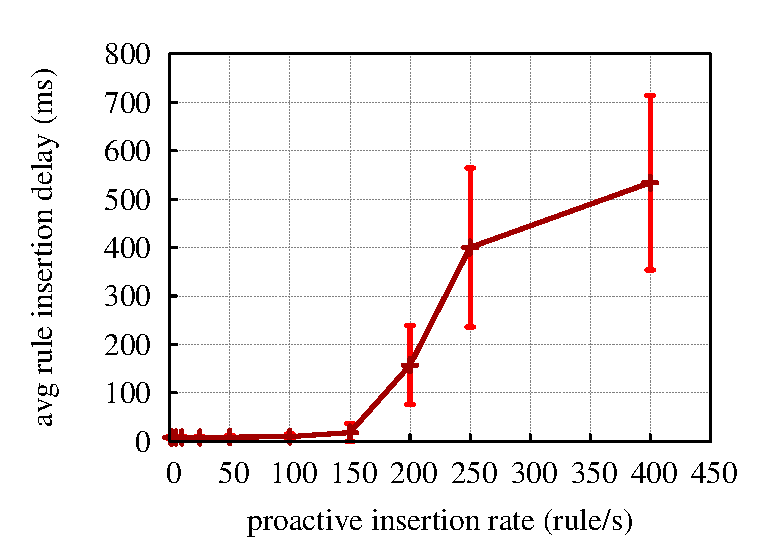
\includegraphics[width=.3\linewidth]{./figs/bcm_insertion_rate_effects_table100_rule300.eps}}\hfill
\subfloat[default table occupancy 100, insert another 700 rules\label{fig:bcm_outbound_rate_effect_3}]
  {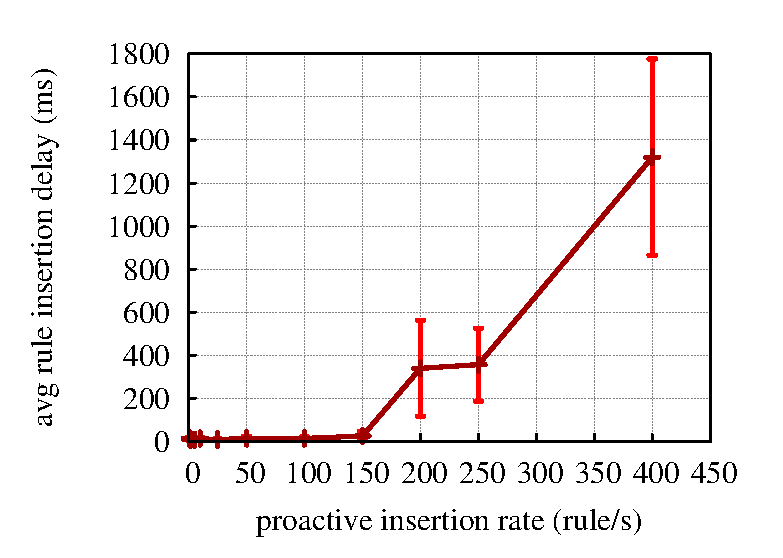
\includegraphics[width=.3\linewidth]{./figs/bcm_insertion_rate_effects_table100_rule700.eps}}\hfill
\subfloat[default table occupancy 400, insert another 50 rules\label{fig:bcm_outbound_rate_effect_4}]
  {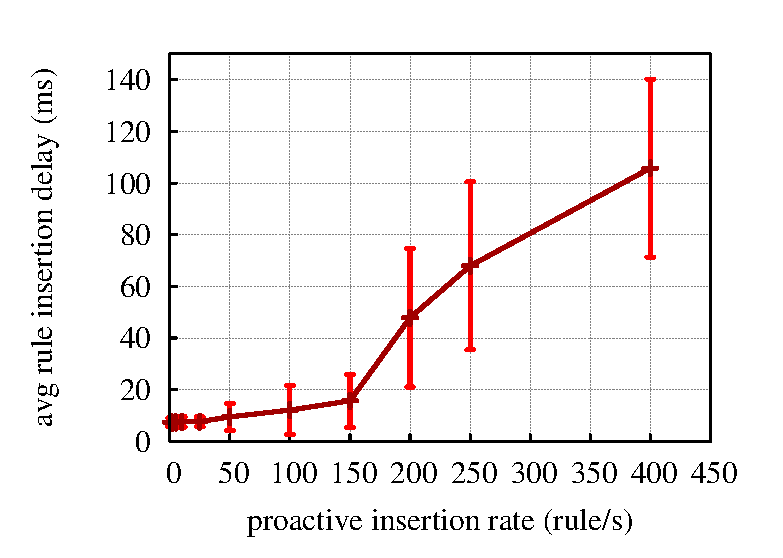
\includegraphics[width=.3\linewidth]{./figs/bcm_insertion_rate_effects_table400_rule50.eps}}\hfill
\subfloat[default table occupancy 400, insert another 200 rules\label{fig:bcm_outbound_rate_effect_5}]
  {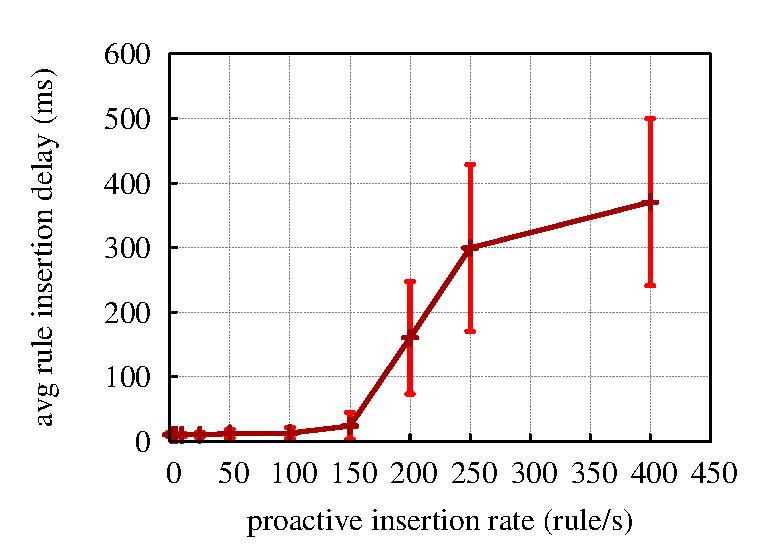
\includegraphics[width=.3\linewidth]{./figs/bcm_insertion_rate_effects_table400_rule200.eps}}\hfill
\subfloat[default table occupancy 400, insert another 400 rules\label{fig:bcm_outbound_rate_effect_6}]
  {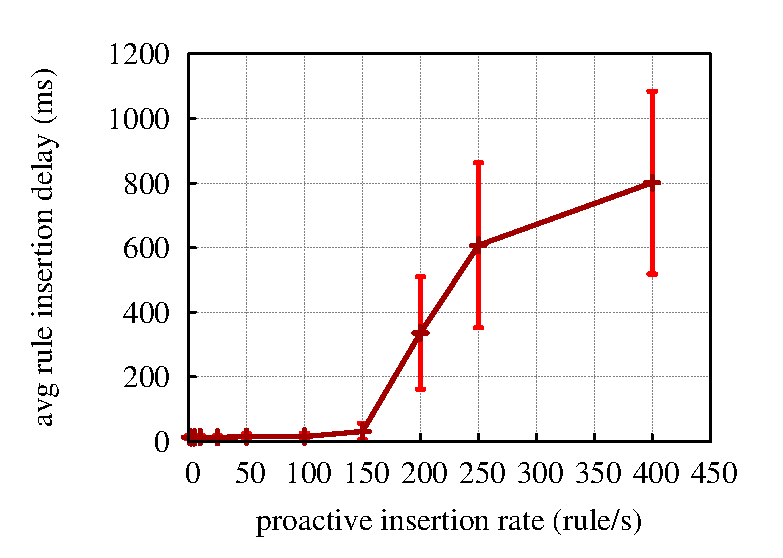
\includegraphics[width=.3\linewidth]{./figs/bcm_insertion_rate_effects_table400_rule400.eps}}
\caption{B3.1, 3.2 and 3.3: Outbound delay on Broadcom switch. Insertion rate effects. Averaged on 5 rounds. Same priority. Measured using simple openflow rules (i.e., just vary destination IP).}
\end{figure*}



%%one insertion rate, one subfigure

\begin{figure*}
\subfloat[Insertion rate = 1/s\label{fig:bcm_outbound_test1}]
  {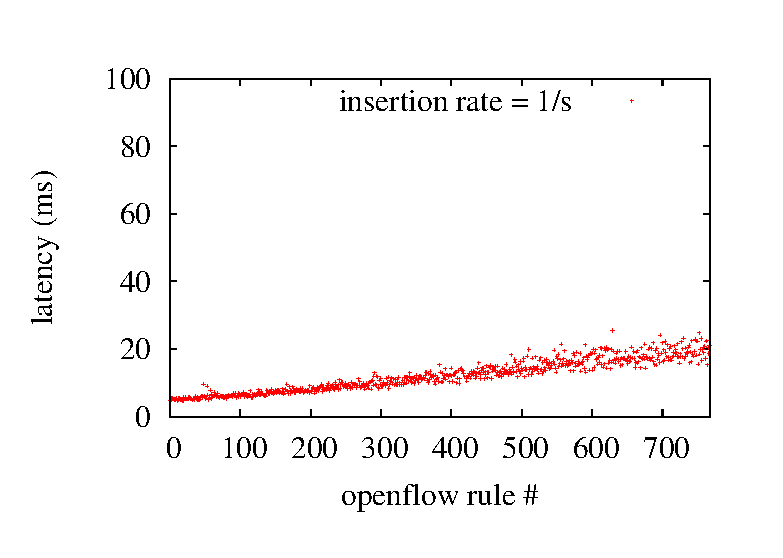
\includegraphics[width=.3\linewidth]{./figs/bcm_same_pri_outbound_rate1.eps}}\hfill
\subfloat[Insertion rate = 10/s\label{fig:bcm_outbound_test2}]
  {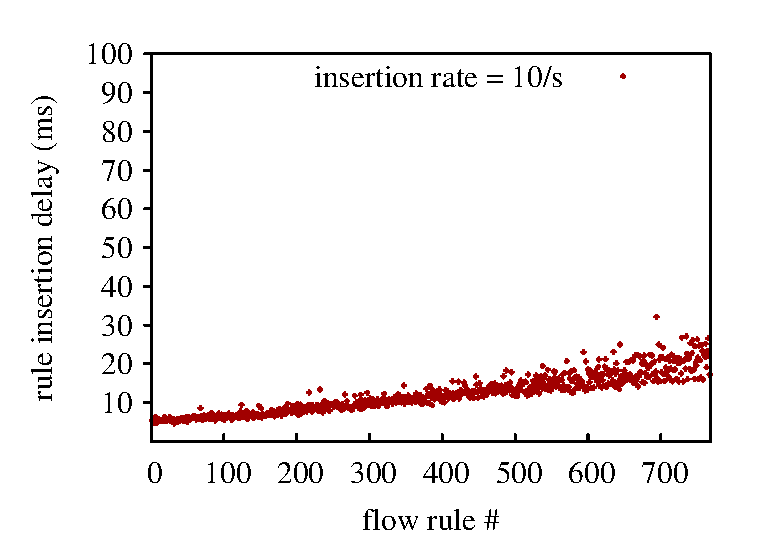
\includegraphics[width=.3\linewidth]{./figs/bcm_same_pri_outbound_rate10.eps}}\hfill
\subfloat[Insertion rate = 50/s\label{fig:bcm_outbound_test3}]
  {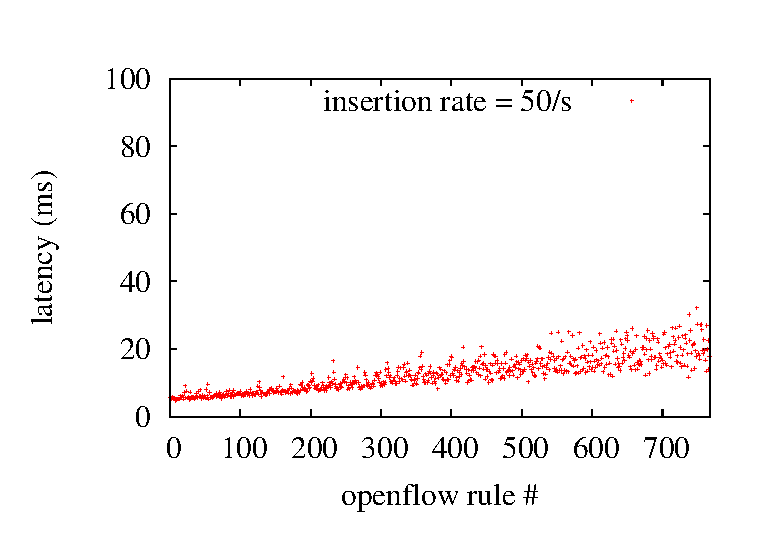
\includegraphics[width=.3\linewidth]{./figs/bcm_same_pri_outbound_rate50.eps}}\hfill
\subfloat[Insertion rate = 100/s\label{fig:bcm_outbound_test4}]
  {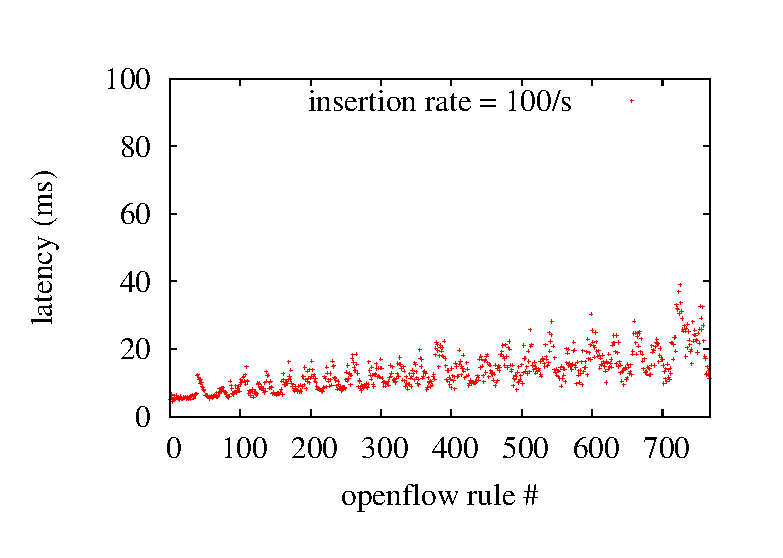
\includegraphics[width=.3\linewidth]{./figs/bcm_same_pri_outbound_rate100.eps}}\hfill
\subfloat[Insertion rate = 150/s\label{fig:bcm_outbound_test5}]
  {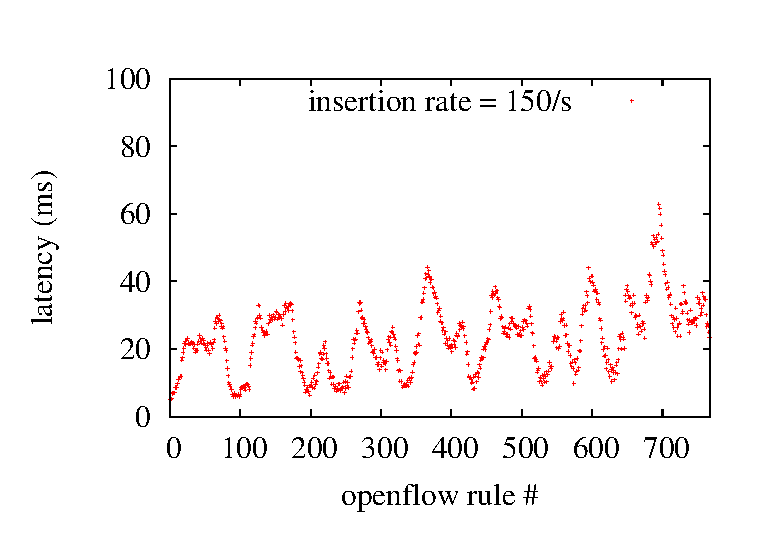
\includegraphics[width=.3\linewidth]{./figs/bcm_same_pri_outbound_rate150.eps}}\hfill
\subfloat[Insertion rate = 200/s\label{fig:bcm_outbound_test6}]
  {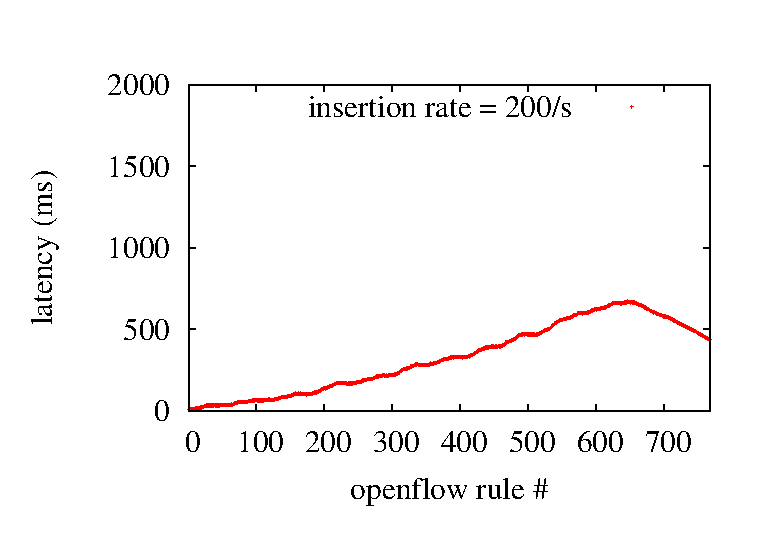
\includegraphics[width=.3\linewidth]{./figs/bcm_same_pri_outbound_rate200.eps}}
\caption{Outbound delay on Broadcom switch. Controlled-rate mode. Averaged on 5 rounds. Measured using simple openflow rules. All rules have the same priority.}
\end{figure*}
